%!TEX root = ../Hardtung_BA_SoSe20.tex

\section{Origrammer}
\label{sec:origrammer}

This section will provide a more detailed overview over the Origrammer. Its parts will be explained and a typical workflow will be shown. Figure \ref{fig:origrammerMain} shows the user interface of the Origrammer, which is split up into five major parts.

\begin{figure}[htbp]
	\centering
	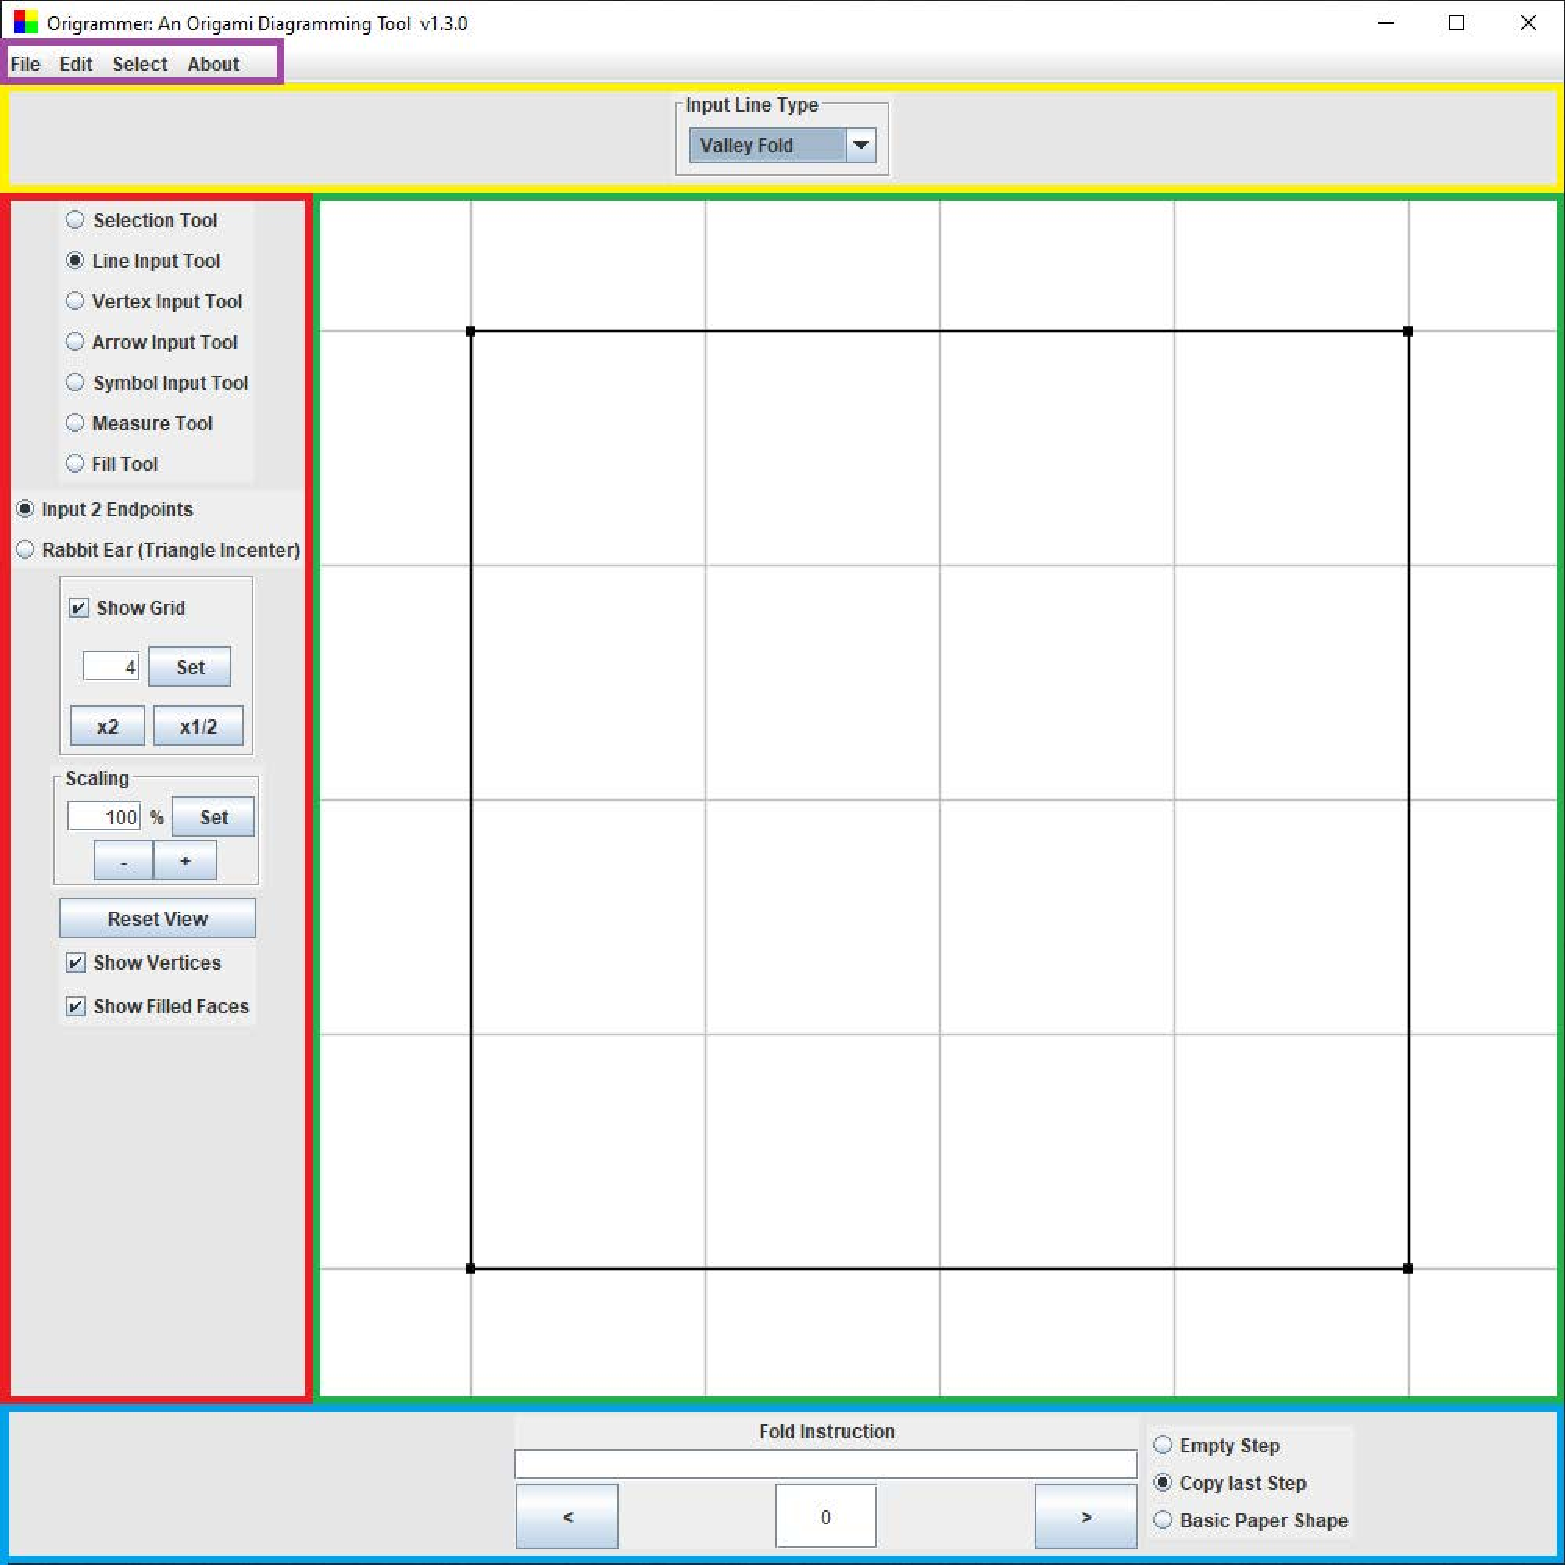
\includegraphics[width=0.8\textwidth]{OrigrammerMainParts}
	\caption{Menu Bar (Purple), Top Panel (Yellow), Side Panel (Red), Editing Panel (Green), Navigation Panel (Blue)}
	\label{fig:origrammerMain}
\end{figure}

\subsection{Menu Bar}

The Menu Bar offers fast and easy access to diagram wide functions. Under \texttt{File}, the user can create a new diagram, open an already existing Origrammer diagram, save a diagram, and \emph{export a diagram to a different format (not yet fully implemented)}. When creating a new diagram, the following panel appears, in which several settings for the diagram can be adjusted.

\begin{figure}[htbp]
	\centering
	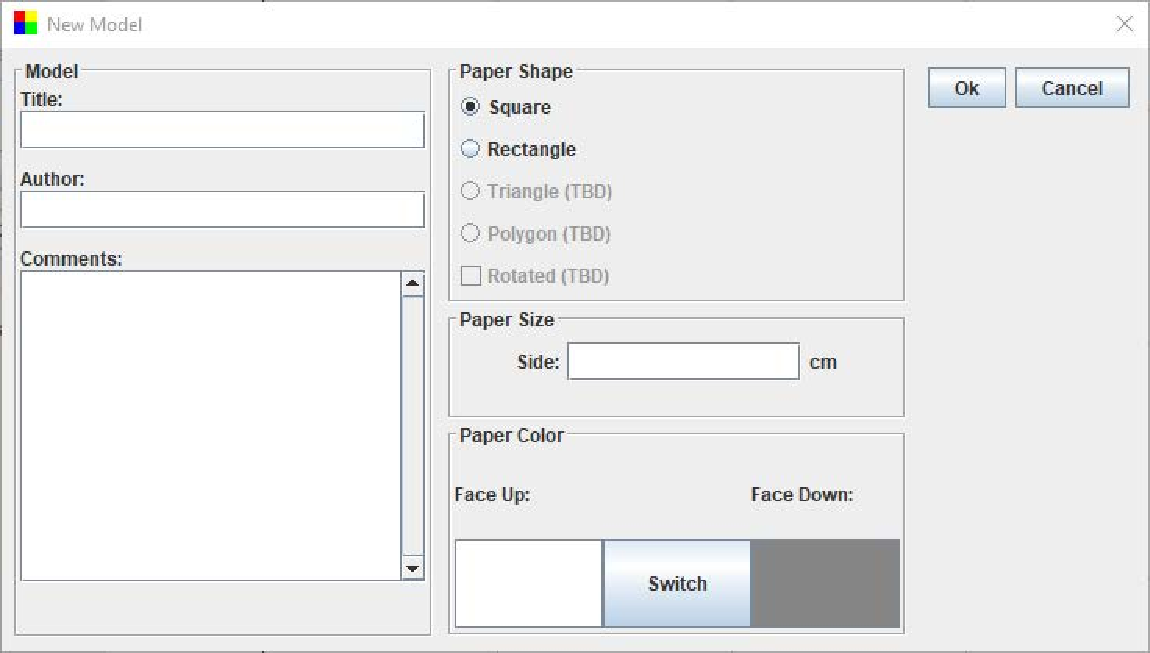
\includegraphics[width=0.72\textwidth]{newDiagram}
	\caption{Options when creating a new diagram}
	\label{fig:newDiagram}
\end{figure}

\newpage
The user is able to provide a \texttt{title}, an \texttt{author}, and \texttt{additional comments} (e.g. regarding copyright information). Additionally, paper related settings can be changed. The required paper shape can be defined (square, rectangle, triangle, polygon, or pre-rotated), a recommended paper size can be provided, and colours for both sides of the paper can be specified.

After confirming the settings for the new diagram, the paper outline of the first diagram step appears on the \ref{sec:editingPanel} Editing Panel.

The next button on the Menu Bar (\texttt{Edit}) includes the typical editing features \texttt{Undo} (Ctrl+Z), \texttt{Redo} (Ctrl+Y), \texttt{Cut} (Ctrl+X), \texttt{Copy} (Ctrl+C), \texttt{Paste} (Ctrl+V), and \texttt{Delete} selection (Delete). Additionally, the previously specified diagram information can be changed at any point under \texttt{Model Preferences} and some Origrammer-wide options can be adjusted under \texttt{Origrammer Preferences} (see Fig. \ref{fig:origrammerPreferences}).

\begin{figure}[htbp]
	\centering
	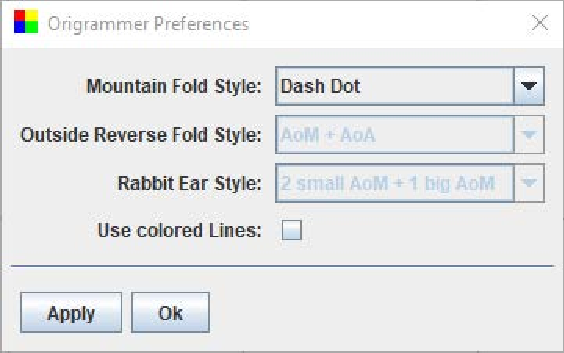
\includegraphics[width=0.45\textwidth]{origrammerPreferences}
	\caption{Origrammer Preferences}
	\label{fig:origrammerPreferences}
\end{figure}

Lastly, under the \texttt{Select} button of the Menu Bar, the user can \texttt{Select all} (Ctrl+A) or \texttt{Unselect all} (Ctrl+Shift+A) objects on a given diagram step.

\newpage
\subsection{Editing Panel}
\label{sec:editingPanel}

The Editing Panel shows the current diagram step that is being worked on. All lines, arrows, and other symbols are being placed and edited here and all tools and input functions can then be used on the Editing Panel.

\subsection{Side Panel}
\label{sec:sidePanel}

All major input tools and adjustments of the Editing Panel are displayed on the Side Panel. The input tools consist of the \texttt{Selection Tool,} the \texttt{Line Input, Vertex Input, Arrow Input, Symbol Input, Measure Tool,} and \texttt{Fill Tool}.

Through the \texttt{Selection Tool}, the user can select, move, and edit already placed objects on a diagram step. The \texttt{Line, Vertex, Arrow,} and \texttt{Symbol Input Tools} make it possible to place the respective objects on a given step. Furthermore, the user can measure the angle and length of lines within the diagram, in order to use these values as input for additional lines. The last tool is the \texttt{Filling Tool}, which offers the function to colour parts of the paper, according to the specified paper colour.

Furthermore, the options for the assisting grid of the Editing Panel can be changed, the scaling can be adjusted to see more detailed parts of a diagram step, and the rendering for vertices and the coloured faces of the diagram can be turned off.

\subsection{Top Panel}
\label{sec:topPanel}

After choosing a tool from the Side Panel, the respective input/editing options of the activated tool are being displayed on the Top Panel. These can be for example sliders for rotations, check boxes for mirroring a symbol, combo boxes for choosing different line/arrow types, and other things.


\subsection{Navigation Panel}
\label{sec:navigationPanel}

The Navigation Panel makes it possible to move through the individual diagram steps, as well as to create new ones. When creating a new step, the user has three different options. The new step can either be completely empty, only consist of the original paper outlines, or can be a simple copy of the previous step.

This is also the area, where the user can write down the textual folding instructions for a given step.
